\documentclass[
  captions=tableheading,  % Tabellenüberschriften
  titlepage=firstiscover, % Titelseite ist Deckblatt
]{scrartcl}

\usepackage{datetime2}

% Paket float verbessern
\usepackage{scrhack}

% Warnung, falls nochmal kompiliert werden muss
\usepackage[aux]{rerunfilecheck}

% unverzichtbare Mathe-Befehle
\usepackage{amsmath}
% viele Mathe-Symbole
\usepackage{amssymb}
% Erweiterungen für amsmath
\usepackage{mathtools}

\usepackage{amsthm}


% Fonteinstellungen
\usepackage{fontspec}
% Latin Modern Fonts werden automatisch geladen
% Alternativ zum Beispiel:
%\setromanfont{Libertinus Serif}
%\setsansfont{Libertinus Sans}
%\setmonofont{Libertinus Mono}

% Wenn man andere Schriftarten gesetzt hat,
% sollte man das Seiten-Layout neu berechnen lassen
\recalctypearea{}

% deutsche Spracheinstellungen
\usepackage[ngerman]{babel}

\usepackage{thmtools}

\usepackage[
  math-style=ISO,    % ┐
  bold-style=ISO,    % │
  sans-style=italic, % │ ISO-Standard folgen
  nabla=upright,     % │
  partial=upright,   % ┘
  warnings-off={           % ┐
    mathtools-colon,       % │ unnötige Warnungen ausschalten
    mathtools-overbracket, % │
  },                       % ┘
]{unicode-math}

% traditionelle Fonts für Mathematik
\setmathfont{Latin Modern Math}
% Alternativ zum Beispiel:
%\setmathfont{Libertinus Math}

\setmathfont{XITS Math}[range={scr, bfscr}]
\setmathfont{XITS Math}[range={cal, bfcal}, StylisticSet=1]

% Zahlen und Einheiten
\usepackage[
  locale=DE,                   % deutsche Einstellungen
  separate-uncertainty=true,   % immer Unsicherheit mit \pm
  per-mode=symbol-or-fraction, % / in inline math, fraction in display math
]{siunitx}



% chemische Formeln
\usepackage[
  version=4,
  math-greek=default, % ┐ mit unicode-math zusammenarbeiten
  text-greek=default, % ┘
]{mhchem}

% richtige Anführungszeichen
\usepackage[autostyle]{csquotes}

% schöne Brüche im Text
\usepackage{xfrac}

% Standardplatzierung für Floats einstellen
\usepackage{float}
\floatplacement{figure}{htbp}
\floatplacement{table}{htbp}

% Floats innerhalb einer Section halten
\usepackage[
  section, % Floats innerhalb der Section halten
  below,   % unterhalb der Section aber auf der selben Seite ist ok
]{placeins}

% Seite drehen für breite Tabellen: landscape Umgebung
\usepackage{pdflscape}

% Captions schöner machen.
\usepackage[
  labelfont=bf,        % Tabelle x: Abbildung y: ist jetzt fett
  font=small,          % Schrift etwas kleiner als Dokument
  width=0.9\textwidth, % maximale Breite einer Caption schmaler
]{caption}
% subfigure, subtable, subref
\usepackage{subcaption}

% Grafiken können eingebunden werden
\usepackage{graphicx}

% schöne Tabellen
\usepackage{booktabs}

% Verbesserungen am Schriftbild
\usepackage{microtype}


\usepackage{listings}

% Hyperlinks im Dokument
\usepackage[
  german,
  unicode,        % Unicode in PDF-Attributen erlauben
  pdfusetitle,    % Titel, Autoren und Datum als PDF-Attribute
  pdfcreator={},  % ┐ PDF-Attribute säubern
  pdfproducer={}, % ┘
]{hyperref}
% erweiterte Bookmarks im PDF
\usepackage{bookmark}

% Trennung von Wörtern mit Strichen
\usepackage[shortcuts]{extdash}

\usepackage{cleveref}

\DeclarePairedDelimiter{\bra}{\langle}{\rvert}
\DeclarePairedDelimiter{\ket}{\lvert}{\rangle}
% <name> <#arguments> <left> <right> <body>
\DeclarePairedDelimiterX{\braket}[2]{\langle}{\rangle}{
#1 \delimsize| #2
}


\author{%
  Yanick Sebastian Kind\\%
  \href{mailto:yanick.kind@udo.edu}{yanick.kind@udo.edu}%
}

\title{Zusammenfassung zur Vorlesung Gruppentheorie in der Physik I}
\date{\today}

\begin{document}

\maketitle

\tableofcontents
\newpage
\section{Ergänzen}
\begin{itemize}
  \item Iso/Homomorphismus
  \item Permutationsgruppe
  \item triviale Darstellung als Isomorphismus
  \item vll. noch Kristallstruktur und Blochtheorem 
  \item wichtigen Liegruppen und dessen Mannigfaltigkeit
  \item Sachen von Henry
  \item Mannigfaltigkeiten verbessern evtl. Bilder
  \item Hakenregel  
  \item Klassifizierung der Lorentz-Trafos (eigentlich, orthochron)
  \item Ab Darstellung eines Viervektors als hermitesche 2 kreuz 2 Matrix recherchieren.
  \item Ende der Vorlesung 11 mit den Dirac-Spinoren und der Dirac-Gleichung
\end{itemize}
\section{Abstrakte Gruppentheorie}
\subsection{Definition: Gruppe}
  Eine Menge $\symcal{G} = \{A_1, A_2,A_3,...\}$ bildet eine Gruppe, wenn mit einer Gruppenverknüpfung $*$ folgende vier Eigenschaften erfüllt sind:
  \begin{enumerate}
    \item \textbf{Abgeschlossenheit}: Mit $A_i, A_j \in \symcal{G}$ folgt $A_i * A_j = A_k \in \symcal{G}$, d.h. die Verknüpfung zweier 
    Elemente ergibt wieder ein Element der Gruppe.
    \item \textbf{Assoziativität}: Es gilt mit $A_i, A_j, A_k \in \symcal{G}$, dass $(A_i * A_j) * A_k = A_i * (A_j*A_k)$.
    \item \textbf{Neutrale Element}: Es exestiert ein eindeutiges Element $E\in \symcal{G}$ mit $E * A_i = A_i * E  = A_i$.
    \item \textbf{Inverse Element}: Zu jedem Element $A_i \in \symcal{G}$ exestiert ein eindeutiges inverses Element $A_i^{-1}$,
      so dass $A_i^{-1} * A_i = A_i * A_i^{-1} = E$ gilt.
  \end{enumerate}
\subsubsection{Endliche Gruppe}
Eine Gruppe mit einer endlichen Anzahl an Elementen heißt endliche Gruppe.
Eine Gruppe $\symcal{G} = \{ E, A_2, \ldots, A_h \} $ ist eine endliche Gruppe der Ordnung $h$.
Man schreibt auch $|\symcal{G}| = h$.
\footnote{Im Folgenden wird das Symbol der Verknüpfung und die Angabe, dass ein Element ein Element
einer Gruppe ist, weggelassen, sofern es eindeutig ist.}
\subsection{Multiplikationstabelle}
Die Multiplikationstabelle gibt einfach an, welche Verknüpfungen welches Gruppenelement ergeben.
Bsp. Symmetrische Gruppe $S_3$:
\[
    \begin{tabular}{>{$}l<{$}|*{6}{>{$}l<{$}}}
    ~   & e   & a   & a^2 & b   & c   & d   \\
    \hline\vrule height 12pt width 0pt
    e   & e   & a   & a^2 & b   & c   & d   \\
    a   & a   & a^2 & e   & c   & d   & b   \\
    a^2 & a^2 & e   & a   & d   & b   & c   \\
    b   & b   & d   & c   & e   & a^2 & a   \\
    c   & c   & b   & d   & a   & e   & a^2 \\
    d   & d   & c   & b   & a^2 & a   & e   \\
    \end{tabular} 
\]
\subsubsection{Rearrangement Theorem}
Sallop gesagt: In jeder Zeile und Spalte einer Multiplikationstabelle kann ein Gruppenelement nur einmal auftreten.\\
Mathematisch: In der Sequenz $EA_k, A_2A_k, \cdots , A_h A_k$ kommt jedes Element $A_i$ nur einmal vor.
\subsection{Zyklische Gruppe}
Bei einer zyklischen Gruppe kann jedes Element durch mehrfacher Multiplikation eines Elements reproduziert werden, so dass
sich jede zyklische Gruppe $\symcal{G}$ als 
\begin{equation*}
  \symcal{G} = \{ X, X^2, \ldots, X^n = E \}
\end{equation*}
schreiben lässt, wobei die Ordnung die Periode der zyklischen Gruppe ist (Bsp.: Translationsgruppe eines Kirstalls)
\subsection{Untergruppen und Nebenklassen}
Sei $\symcal{S}  = \{E, S_2, \ldots, S_g \}$ eine Untergruppe der Ordnung $g$ der Gruppe $\symcal{G}$
der Ordnung $h$, dann ist 
\begin{equation*}
  \symcal{S}X = \{ EX, S_2X, \ldots, S_g X\}
\end{equation*}
eine rechte Nebenklasse von $\symcal{S}$ (linke Nebenklasse analog).
Wäre $X \in \symcal{S}$, dann wäre $X\symcal{S}$ wieder $\symcal{S}$ selbst und damit enthält
eine Nebenklasse kein einziges Element der Untergruppe.\\
\subsubsection{Satz: Disjunkheit oder Gleichheit}
Zwei (linke oder rechte) Nebenklassen $X\symcal{S}, Y\symcal{S}$ einer Untergruppe $\symcal{S}$ sind entweder 
disjunkt oder gleich.
\subsubsection{Satz: Index einer Untergruppe}
Die Ordnung einer Untergruppe $\symcal{S}$ von $\symcal{G}$, wobei 
$|\symcal{S}| = g$ und $|\symcal{G}| = h$ gilt, muss ein ganzzahliger Teiler von $h$ sein, so dass 
\begin{equation*}
  \frac{h}{g} = l \in \symbb{Z}
\end{equation*}
gilt.
Dabei wird $l$ der Index der Untergruppe $\symcal{S}$ in $\symcal{G}$ genannt.
\subsection{Konjugierte Elemente und Klassen}
Zwei Elemente $A, B$ sind zueinander konjugiert, wenn 
\begin{equation*}
  B = X A X^{-1}
\end{equation*}
gilt.
Damit folgt, dass wenn $C$ und $B$ zu $A$ konjugiert sind, dass auch $B$ und $C$ zueinander konjugiert sind.
\subsubsection{Konjugationsklasse}
Alle Elemente einer Gruppe $\symcal{G}$, die zueinander konjugiert sind, bilden eine Konjugationsklasse
\begin{equation*}
  \symcal{G} A = \{BAB^{-1} | B \in \symcal{G} \},
\end{equation*}
wobei A ein beliebiges Element der Konjugationsklasse ist.
\subsection{Normalteiler und Faktorgruppen}
\subsubsection{Definition: Normalteiler}
\label{def:normalteiler}
Eine Untergruppe $\symcal{S}$ einer Gruppe $\symcal{G}$, die nur aus kompletten Klassen besteht,
heißt \textbf{Normalteiler} oder \textbf{invariante Untergruppe}.
Mit einer komplette Klasse meint man, dass, wenn $A$ in  $\symcal{S}$ liegt, alle Elemente $XAX^{-1}$ in $\symcal{S}$ liegen,
selbst wenn $X\in\symcal{G}$ nicht in $\symcal{S}$ liegt.
Solche eine Untergruppe heißt invariant, da es unter Konjugation mit einem beliebigen Element 
von $\symcal{G}$ invariant ist.
\subsubsection{Einschub: Komplexe}
Ein Komplex
\begin{equation*}
  \symcal{K} = \{ K_1, \ldots, K_n \} 
\end{equation*}
ist eine Menge von Gruppenelementen unter Vernachlässigung der Reihenfolge.
Eine Multiplikation mit einen beliebigen Element $X$ ist durch $\symcal{K}X = \{ K_1 X, \ldots, K_n X \}$ gegeben.
Die Multiplikation zweier Komplexe $\symcal{K} = \{ K_1, \ldots, K_n \} $ und $\symcal{K}' =  \{ K_1', \ldots, K_m' \} $ ist durch 
$\symcal{K}\symcal{K'} = \{ K_1 K_1', K_2 K_1', \ldots, K_1 K_2', K_1 K_3', \ldots, K_n K_m'  \} $ gegeben.
Doppelte Elemente werden, wie es bei einer Menge üblich ist, nicht mitgezählt.

\subsubsection{Satz: Nebenklasse einer invarianten Untergruppe}
Aus der Definition \ref{def:normalteiler} folgt
\begin{equation*}
  X\symcal{S}X^{-1} = \symcal{S} \iff X\symcal{S} = \symcal{S}X,
\end{equation*}
womit die rechte gleich der linken Nebenklasse einer invarianten Untergruppe ist.
\subsubsection{Definiton: Faktorgruppe}
Eine invariante Untergruppe $\symcal{S}$ einer Gruppe $G$ bildet mit all ihren $l-1$ Nebenklassen eine Faktorgruppe 
\begin{equation*}
  \sfrac{\symcal{G}}{\symcal{S}} = \{S, \symcal{S}X_1, \symcal{S}X_2, \ldots, \symcal{S}X_{l-1} \},
\end{equation*}
wobei die invariante Untergruppe $\symcal{S}$ das Einselement bildet.
Die Ordnung der Faktorgruppe entspricht $\sfrac{|\symcal{G}|}{|\symcal{S}|}$.
\section{Darstellungstheorie}
Wir haben uns ausschließlich mit Matrizendarstellungen beschäftigt.
\subsection{Definition: Darstellung}
Bei einer Darstellung $\symup{\Gamma}$ wird jedem Gruppenelement eine quadratische Matrix zugeordnet
\begin{equation*}
  \symup{\Gamma}(A) : \quad \symcal{V} \to \symcal{V}.
\end{equation*}
Der Vektorraum $\symcal{V}$ wird Darstellungsraum genannt, wobei $\text{Dim}(\symcal{V}) = d$ die Dimension der Darstellung ist.
Eine lineare Darstellung $\symup{\Gamma} (A)$ von $\symcal{G}$ ist ein Homomorphismus der Gruppe GL$(\symcal{V})$
\begin{equation*}
  \symup{\Gamma}(A) \symup{\Gamma}(B) = \symup{\Gamma}(AB), \quad A,B \in \symcal{G}.
\end{equation*} 
Das Einselement wird durch die Einheitsmatrix dargestellt.
\subsection{Definition: Äquivalente Darstellung}
Eine andere Darstellung lässt sich durch eine Ähnlichkeitstransformation gewinnen
\begin{equation*}
  \symup{\Gamma}'(A) = S^{-1} \symup{\Gamma} (A) S \implies \symup{\Gamma}'(A) \symup{\Gamma}'(B) = \symup{\Gamma}'(AB).
\end{equation*}
Die Darstellungen $\symup{\Gamma}$ und $\symup{\Gamma}'$ sind äquivalent.
\subsection{(Ir)reduzibilität}
Die direkte Summe von zwei Darstellungen 
\begin{equation*}
  \symup{\Gamma} (A) = 
  \begin{pmatrix}
    \symup{\Gamma}^1 (A)  & 0           \\
    0             & \symup{\Gamma}^2(A)
  \end{pmatrix}
  , \quad \symup{\Gamma} (A) = \symup{\Gamma}^1 (A)\bigoplus \symup{\Gamma}^2(A)
\end{equation*}
ist eine weitere Form von Redundanz.
Lässt sich eine Darstellung durch eine globale Ähnlichkeitstransformation auf eine Blockdiagonale
bringen, ist sie reduzibel, sonst irreduzibel.
\subsection{Satz: unitäre Darstellungen}
Jede Darstellung lässt sich mit Hilfe einer Ähnlichkeitstransformation auf eine 
unitäre Darstellung abgebilden. 
Vorgehen: Konstruiere hermitesche Matrix 
${\mathbf{H} = \sum_i^h \symup{\Gamma}(A_i) \symup{\Gamma} (A_i)^\dagger}$. 
Dann diese diagonalisieren mit unitärer Trafo 
$\mathbf{d} = \mathbf{U}^{-1} \mathbf{H} \mathbf{U}$. 
Somit ist die Darstellung 
\begin{equation*}
  \symup{\Gamma}^{'}(A_j) = \mathbf{d^{-\frac{1}{2}}} \mathbf{U}^{-1} \symup{\Gamma}(A_j) \mathbf{U} \mathbf{d}^{\frac{1}{2}}
\end{equation*}
unitär.
\subsection{Schur'sches Lemma}
Jede Matrix, welche mit allen Matrizen einer irreduziblen Darstellung kommutiert,
muss ein Vielfaches von der Einheitsmatrix (sog. konstante Matrix) sein. 
Wenn somit eine nicht-konstante Matrix mit mindestens einer Matrix einer Darstellung kommutiert, 
ist diese Darstellung reduzibel.
\subsubsection{Alternative Formulierung}
Gegeben seien zwei Darstellungen mit $\text{Dim}(\symup{\Gamma}^1(A)) = d_1$ und $\text{Dim}(\symup{\Gamma}^2(A)) = d_2$.
Wenn dann mit einer beliebigen Matrix $\mathbf{M}$
\begin{equation*}
  \mathbf{M}\symup{\Gamma}^1(A) = \symup{\Gamma}^2(A) \mathbf{M}
\end{equation*}
gilt, dann muss (i) bei $d_1 \neq d_2$ $\mathbf{M} = \mathbf{0}$ oder (ii) bei $d_1 = d_2$ entweder 
$\mathbf{M} = \mathbf{0}$ oder $|\mathbf{M}| \neq 0$ gelten.
Aus letzterem folgt $\symup{\Gamma}^1(A) = \mathbf{M} \symup{\Gamma}^2(A) \mathbf{M}^{-1} $, womit 
die Darstellungen äquivalent sind.
\subsection{Orthogonalitätstheorem}
\label{sub:orth}
Bei Betrachtung \textbf{nicht-äquivalenter}, unitärer, irreduziblen Darstellungen gilt
\begin{equation*}
  \sum_R \symup{\Gamma}^i(R)^*_{\mu \nu}\symup{\Gamma}^j(R)_{\alpha \beta} = \frac{h}{d_i} \delta_{ij}\delta_{\mu \alpha}\delta_{\nu \beta}.
\end{equation*}
Geometrische Interpretation: die Gruppelemente $R = E, A_2, \ldots, A_h$ spannen einen 
$h$-dimensionalen \enquote{Gruppenelement}-Vektorraum auf.
Jeder Vektor in diesem Raum hat drei Indizes, $i, \mu, \nu$.
Diese Vektoren sind orthogonal zueinander.
\subsection{Satz von Burnside}
Aus der geometrischen Interpretation des Orthogonalitätstheorems \ref{sub:orth} folgt 
mit $d_i$ als Dimension der $i$-ten irreduziblen Darstellung der Gruppe $\symcal{G}$ direkt
\begin{equation*}
  \sum_i d_i^2 = |\symcal{G}|,
\end{equation*}
da es zu jeder Darstellung $\symup{\Gamma}^i$ $d_i^2$ verschiedene Vektoren gibt. 
Das heißt, dass in Summe in diesem Vektorraum $\sum_i d_i^2$ verschiedene Vektoren exestieren.
Da in einem $h$-dimensionalen Vektorraum nur maximal $h$ zueinander orthogonale Vektoren exestieren können,
folgt $\sum_i d_i^2 \leq h = |\symcal{G}|$. 
Die eindeutige Gleichheit wird z.B. im Tinkham bewiesen.
\subsection{Definition: Charakter}
Der Charakter einer Darstellung $\symup{\Gamma}^i(R)$ ist die Menge
der $h$ Zahlen $\chi^i(E), \chi^i(A_2), \ldots, \chi^i(A_h)$ mit
\begin{equation*}
  \chi^i(R) = \text{Tr}(\symup{\Gamma}^i(R)) = \sum_j^{d_i} \symup{\Gamma}^i(R)_{jj}.
\end{equation*}
Die Spur ist unter einer Ähnlichkeitstransformation invariant, so dass äquivalente Darstellungen und 
Elemente innerhalb einer Klasse denselben Charakter besitzen.
Im Folgenden wird der Charakter für die $k$-te Klasse $\symcal{G}_k$ durch $\chi^i(\symcal{G}_k)$ angegeben.
\subsection{Satz: Zeilenorthogonalität}
Wird das Orthogonalitätstheorem genutzt, kann 
\begin{equation*}
  \sum_R \chi^i(R)^* \chi^j(R) = \sum_R \chi^i(\symcal{G}_k)^* \chi^j(\symcal{G}_k) N_k = h \delta_{ij}
\end{equation*}
gezeigt werden, wobei $N_k$ die Anzahl an Elementen in der $k$-ten Klasse ist.
Somit formen die Charaktere der verschiedenen irreduziblen Darstellungen eine Menge von orthogonalen Vektoren 
\begin{equation*}
\chi^i = 
\begin{pmatrix}
  \chi^i(E       )\\
  \chi^i(\symcal{G}_2     )\\
  \ldots          \\
  \chi^i(\symcal{G}_n     )
\end{pmatrix}
\end{equation*}  
in einem $n$-dimensionalen Vektorraum, welcher durch die Klassen $\symcal{G}_k$ aufgespannt wird.
Da die Anzahl der orthogonalen Vektoren die Dimension des Vektorraums nicht übersteigen kann,
darf die Anzahl der Klassen nicht die Anzahl der irreduziblen Darstellungen übersteigen.
Es gilt sogar
\begin{equation*}
  \text{Anzahl Klassen} = \text{Anzahl irreduzible Darstellungen}.
\end{equation*}
\subsection{Charaktertafel}
In den Zeilen stehen die irreduziblen Darstellungen und in den Spalten die Klassen mit 
der Anzahl an Elementen in der jeweiligen Klasse.
\begin{table}
  \centering
  \caption{Charaktertafel der $S_3$}
  \label{tab:some_data}
  \sisetup{table-format=2.0}
  \begin{tabular}{S[table-format=10.0] S[table-format = 1.0] S S}
  \toprule
   & {$\symcal{G}_1$} & {$3\symcal{G}_2$} & {$2\symcal{G}_3$} \\
  \midrule
  {$\symup{\Gamma}^1$} & 1 & 1  & 1   \\
  {$\symup{\Gamma}^2$} & 1 & -1 & 1   \\
  {$\symup{\Gamma}^3$} & 2 & 0  & -1  \\
  \bottomrule
  \end{tabular}
  \end{table}
\subsection{Satz: Spaltenorthogonalität}
Für irreduzible Darstellungen $\chi^i$ und $\chi^j$ gilt
\begin{equation*}
  \sum_i \chi^i(\symcal{G}_k)^* \chi^i(\symcal{G}_l) = \frac{h}{N_k} \delta_{kl}.
\end{equation*}
\subsection{Dekomposition von reduziblen Darstellungen}
Bringe die Darstellung erst auf blockdiagonale Form
\begin{equation*}
  \symup{\Gamma} (R) = 
  \begin{pmatrix}
    \symup{\Gamma}^1 (R)  &       &    \\
    & \!\!\!\!\!\! \symup{\Gamma}^2(R) &  \\
    & & \ddots \quad \quad
  \end{pmatrix}
  , \quad \symup{\Gamma} (R) = \symup{\Gamma}^1 (R)\bigoplus \symup{\Gamma}^2(R) \bigoplus \cdots
\end{equation*}
mit den irreduziblen Darstellungen auf der Diagonale.
Somit ist die Spur der reduziblen Darstellung die Summe der Spuren der irreduziblen Darstellungen
\begin{equation*}
  \chi_{\text{red}} (R) = \sum_i a_i \chi_{\text{irred}}^i(R),
\end{equation*}
wobei der Koeffizient $a_i$ angibt, wie oft die $i$-te irreduzible Darstellung auf der 
Diagonale vorkommt.
Durch Anwendung des Orthogonalitätstheorems \ref{sub:orth}, sind die Koeffizienten eindeutig 
durch den Charakter der reduziblen Darstellung bestimmt.
\begin{equation}
  a_i = \frac{1}{h} \sum_k N_k \chi_{\text{irred}}^i (\symcal{G}_k)^* \chi_{\text{red}} (\symcal{G}_k) . \label{eqn:decomp}
\end{equation}
\subsection{Reguläre Darstellung}
Hier schiebt man einfach die Elemente in der Multiplikationstabelle so rum, so dass 
auf der Hauptdiagonalen das Einselement liegt. 
Wenn man nun die reguläre Darstellung eines Elements bestimmen möchte, schaut man in der 
Multiplikationstabelle, wo dieses Element als Resultät der Multiplikationen steht.
Damit bekommt die Matrix der regulären Darstellung eine $1$ als Eintrag an dieser Stelle.
\[
    \begin{tabular}{>{$}l<{$}|*{6}{>{$}l<{$}}}
    ~       & E   & A & B & C & D & F   \\
    \hline\vrule height 12pt width 0pt
    E       & E   & A & B & C & D & F\\
    A^{-1}  & A   & E & D & F & B & C\\
    B^{-1}  & B   & F & E & D & C & A\\
    C^{-1}  & C   & D & F & E & A & B\\
    D^{-1}  & F   & B & C & A & E & D\\
    F^{-1}  & D   & C & A & B & F & E\\
    \end{tabular} 
\]
\begin{equation*}
  \symup{\Gamma}_\text{reg}(A)
  \begin{pmatrix}
    0 & 1 & 0 & 0 & 0 & 0 \\
    1 & 0 & 0 & 0 & 0 & 0 \\
    0 & 0 & 0 & 0 & 0 & 1 \\
    0 & 0 & 0 & 1 & 1 & 0 \\
    0 & 0 & 0 & 0 & 0 & 0 \\
    0 & 0 & 1 & 0 & 0 & 0 
  \end{pmatrix}
\end{equation*}
Aus \begin{equation*}
  \chi_\text{reg} \cdot \chi_\text{irred}^i = 
  \begin{pmatrix}
    h \\
    0 \\
    \cdots
  \end{pmatrix}
  \cdot 
  \begin{pmatrix}
    d_i \\
    x   \\
    \cdots
  \end{pmatrix}
  = h d_i 
\end{equation*}
folgt, dass die reguläre Darstellung \textbf{jede} irreduzible Darstellung genau $d_i$ mal entält (s. Gl. \eqref{eqn:decomp}).
\section{Symmetrieoperationen in der Quantenmechanik}
Ausgangspunkt ist die Schrödingergleichung 
\begin{equation*}
  \hat {H} \Psi_n = E_n^j \Psi_n.
\end{equation*}
Dabei gibt j den Grad der Entartung an.
Ziel ist es nun einen Zusammenhang zwischen den Symmetrieoperationen und der Entartung der Energieniveaus 
zu finden.
\subsection{Wirkung der Symmetrieoperationen auf Wellenfunktionen}
Sei $\hat{P}_R$ eine Symmetrieoperation.
Diese wirkt auf eine Wellenfunktion gemäß
\begin{equation*}
  \hat{P}_R \Psi (\vec{r}) = \Psi(\mathbf{R}^{-1}\vec{r}).
\end{equation*}
Somit kann entweder der Vektor um einen Winkel im mathematisch positiven Drehsinn oder 
das Koordinatensystem um diese Winkel im mathematisch negativen Drehsinn gedreht werden.
Die Symmetrieoperatoren bilden eine Gruppe, die isomorph zu der Gruppe der 
Koordinatentransformationen ist.
\subsection{Symmetrie des Hamiltonoperators}
\label{sub:symmhamil}
Wenn das System und damit auch der Hamiltonian invariant unter einer Symmetrieoperation ist, vertauscht 
der Hamiltonian mit dem Symmetrieoperator und somit gilt 
\begin{equation*}
  \hat{H} \Psi = E_n \Psi \iff 
  \hat{P}_R \hat{H} \Psi = E_n \hat{P}_R \Psi \iff 
  \hat{H} \hat{P}_R \Psi = \hat{H} \Psi' = E_n \Psi',
\end{equation*}
d.h. bei Symmetrien haben verschiedene Zustände die selbe Energie, womit Entartung vorliegt.
\subsection{Die Gruppe der Schrödingergleichung}
\label{sub:schrdgroup}
Sei nun ein Energieniveau $E_n$ $d_n$-fach entartet.
Dann wähle $d_n$ orthonormale Eigenfunktionen, welche zu $E_n$ gehören.
Diese $d_n$ Eigenfunktionen spannen den entarteten Unterraum $\symcal{V} \in \symcal{H}$ 
von dem gesamten Hilbertraum $\symcal{H}$ auf, welcher invariant unter den Symmetrieoperationen, welche 
lineare Abbildungen 
\begin{equation*}
  \hat{P}_R: \quad \symcal{V} \to \symcal{V}
\end{equation*}
sind, ist.
Die Darstellungen sind irreduzibel, da in dem Raum $\symcal{V}$ kein invarianter Unterraum exestiert.
\subsection{Bestimmung einer Darstellung der Symmetriegruppe}
Nach Abschnitt \ref{sub:schrdgroup} erhält man durch Anwendung der Symmetrieoperation auf eine 
Eigenfunktion des entarteten Unterraums eine Linearkombination aller Eigenfunktionen
\begin{equation*}
  \hat{P}_R \Psi_\nu^n = \sum_\kappa \symup{\Gamma}^n(R)_{\kappa \nu} \Psi_\kappa^n .
\end{equation*}
Die Matrixen $\symup{\Gamma}^n(R)$ bilden dann eine irreduzible Darstellung zu der Symmetriegruppe, unter welcher 
der entartete Unterraum mit dem Energiveau $E_n$ invariant ist.
\subsection{Unitarität der Darstellung}
Nur wenn die Eigenfunktionen orthonormiert gewählt werden, sind die Darstellungen unitär.
\subsection{Entartungsgrad}
\begin{equation*}
  \text{Entartungsgrad} = \text{Dimension der irreduziblen Darstellung}
\end{equation*}
\section{Liegruppen}
\begin{enumerate}
\item erfüllen Gruppenaxiome 
\item besitzen eine analytische Mannigfaltigkeit
\item Abstandsbegriff (bilden topologischen Raum, metrischen Raum)
\end{enumerate}
\subsection{Definiton: Liegruppe}
Eine Gruppe $\symcal{G}$ wird Liegruppe genannt, wenn
\begin{enumerate}
  \item $\symcal{G}$ besitzt mindestens eine endliche Darstellung $\symup{\Gamma}(T)$ mit $T \in \symcal{G}$ der Dimension 
  $d$. 
  Definiere einen Abstand 
    \begin{equation*}
      d(T,T') = \sqrt{\sum_{\substack{j=1}{k=1}} \left | \symup{\Gamma}(T)_{jk} - \symup{\Gamma}(T')_{jk} \right |^2  } = d(T',T) > 0
    \end{equation*}
    und somit eine Metrik.
  \item Jedes Element $T$ kann durch $n$ reelle Parameter $\theta = (\theta_1, \ldots, \theta_n)$ angegeben werden.
    $n$ ist dann die Dimension der Liegruppe und die minimale Anzahl an Elementen.
  \item Nähe zum Einselement. Sei $\eta$ vorgegeben, dann gehört zu jedem Punkt $\theta =  (\theta_1, \ldots, \theta_n)$,
    für den $\sum_i^n \theta_i^2 < \eta^2$ gilt, ein Element $T \in \symcal{G}$.
  \item Die Darstellungen $\symup{\Gamma}(T(\theta))$ sind in den Parametern analytisch und somit in eine Potenzreihe entwickelbar.
\end{enumerate}
Die Gruppenelemente $T(\theta)$ sind \enquote{smooth} bzgl. den Parametern. 
Das bedeutet, dass, wenn die Gruppenelemente nah beieinander sind, die Parameter ebenfalls nah beieinander sind.
Ebenfalls soll das Einselement bei $\theta = 0$ liegen
\begin{equation*}
  T(\theta)\big |_{\theta = 0} = E \iff \symup{\Gamma}(T(\theta)) \big |_{\theta = 0} = \mathbb{1} .
\end{equation*}
\subsection{Erzeugenden}
Die $n$ Erzeugenden/Generatoren einer $n$-dimensionalen Liealgebra sind gemäß 
\begin{equation}
  \frac{1}{i} \frac{\partial}{\partial \theta_j} \symup{\Gamma}(T(\theta)) \biggr |_{\theta = 0} = t_j \label{eqn:gen}
\end{equation}
definiert. 
Der Faktor $\sfrac{1}{i}$ ist Konvention.
Wenn man die Darstellungen bis zur ersten Ordnung entwickelt und fordert, dass die Darstellungen 
unitär sind, folgt, dass die Generatoren hermitesch sein müssen. 
\begin{align*}
  \symup{\Gamma}(T(\theta)) &= \symbb{1} + \frac{\partial \symup{\Gamma}(T(\theta))}{\partial \theta_a} \biggr |_{\theta = 0} \theta_a + \symbfcal{O}(\theta^2) 
  = \mathbb{1} + i t_a \theta_a + \symbfcal{O}(\theta^2) \\
  \implies \symup{\Gamma}(T(\theta))\symup{\Gamma}(T(\theta))^{\dagger}  &\approx \mathbb{1} + i \theta_a (t_a - t_a^{\dagger}) \stackrel{!}{=} \mathbb{1} \iff t_a = t_a^{\dagger}
\end{align*}
\subsection{Strukturkonstanten}
Ausgang ist die Gruppeneigenschaft. 
Somit muss mit $T(\theta), T(\theta') \in \symcal{G}$ 
\begin{equation*}
  T(\theta)T(\theta') = T(f(\theta, \theta'))
\end{equation*} gelten.
Es gilt ebenfalls $\theta = \theta_1, \ldots, \theta_n, \; f = f_1, \ldots, f_n$ mit n als Dimension der Gruppe.
Bestimme nun $f(\theta, \theta')$ und entwickle $f$ in die zweite Ordnung.
Dann nochmal die Darstellungen in erste Ordnung entwickeln und dann einen Koeffizientenvergleich machen, womit 
die Bedingung für eine Liealgebra
\begin{equation*}
  [t_a, t_b] = i \sum_c^n f_{ab}^ct_c
\end{equation*}
folgt. 
Die $f_{ab}^c$ als sind Strukturkonstanten,
welche extrem wichtig sind, da diese die gesamte Gruppenmultiplikation zusammenfassen.
\subsection{Exponentielle Parameterisierung}
\label{sub:exp}
Eine inifinitesimale Transformation lässt sich durch eine Reihenentwicklung bis zur ersten Ordnung darstellen.
\begin{equation*}
  \symup{\Gamma}(\symup{d}\theta) = \mathbb{1} + i \sum_a^n t_a \symup{d}\theta_a.
\end{equation*}
Man stelle sich vor, dass eine Transformation in $k$ gleiche Stücke unterteilt wird und diese Teil-Transformationen
$k$ mal ausgeführt werden
\begin{equation*}
  \symup{\Gamma}(\theta) = (\mathbb{1} + i \sum_a^n t_a \symup{d}\theta_a)(\mathbb{1} + i \sum_a^n t_a \symup{d}\theta_a)
  \cdots (\mathbb{1} + i \sum_a^n t_a \symup{d}\theta_a)
  = (\mathbb{1} + i \sum_a^n t_a \symup{d}\theta_a)^k.
\end{equation*}
Um nun eine infinitesimale Transformation zu beschreiben, können wir den Parameter 
$\symup{d}\theta_a$ auch einfach durch $\symup{d}\theta_a = \frac{\theta}{k}$ darstellen und $k$ gegeben
Unendlich laufen lassen.
Um nun aber eine finite Transformation zu erhalten, müssen wir diese inifinitesimale Transformation unendlich oft anwenden.
Damit lässt sich die Transformation als Limite
\begin{equation*}
  \symup{\Gamma}(\theta) = \lim_{k \to \infty} (\mathbb{1} + i \sum_a^n t_a \frac{\theta_a}{k})^k = \symup{e}^{i\sum_a^n t_a \theta_a}
  = \symup{e}^{i\vec{t} \cdot \vec{\theta}}
\end{equation*}
finden, wobei der Übergang zur Exponentialfunktion gemacht wurde.
\subsubsection{Einschub: Name \enquote{Generator}}
Den Namen \enquote{Generator} lässt sich begründen, indem man ein Element der Gruppe als Matrix um die Eins entwickelt, also 
\begin{equation*}
  \symup{\Gamma}(\theta) = \mathbb{1} + \frac{\symup{d}\symup{\Gamma}}{\symup{d} \theta} \big |_{\theta = 0} \theta + 
  \frac{\symup{d^2}\symup{\Gamma}}{\symup{d} \theta^2} \big |_{\theta = 0} \theta^2 + \cdots  = \sum_{n=0}^{\infty}\frac{1}{n!}
  \frac{\symup{d}^n\symup{\Gamma}}{\symup{d} \theta^n} \big |_{\theta = 0} \theta^n .
\end{equation*}
In diese Reihenentwicklung können die Generatoren einfach eingesetzt werden und damit sieht man, dass 
die Generatoren tatsächlich die Transformationen generieren.
\subsection{Lie-Klammern}
Die Erzeugenden erfüllen die Axiome einer Liealgebra, d.h. für die Generatoren $t_a \in \symcal{V}$ ist 
zusätzlich eine Verknüpfung, die Lie-Klammer, 
\begin{align*}
  \symcal{V} * \symcal{V} &\to \symcal{V} \\
  x,y \in \symcal{V}      &\to [x,y] \in \symcal{V}
\end{align*}
definiert, welche die Eigenschaften 
\begin{enumerate}
  \item Biliniarität: $[\alpha x + \beta y, z] = \alpha [x,z] + \beta [y,z]$
  \item $[x,x] = 0$
  \item Jacobi-Identität (zyklische Vertauschung): $[x, [y,z]] + [z,[x,y]] + [y,[z,x]] = 0$
\end{enumerate}
erfüllen.
\subsection{\texorpdfstring{$SO(3)$}{PDFstring}}
S für speziell (Determinante ist eins), O für orthogonal und drei für $3 \times 3$-Matrizen.
Die $SO(3)$ ist eigentlich einfach nur  die Gruppe der Drehungen im $\mathbb{R}^3$.
Die Generatoren $J_i$ können gemäß Gleichung \eqref{eqn:gen} bestimmt werden
\begin{equation*}
  J_1 = 
  \begin{pmatrix}
    0 & 0 & 0   \\
    0 & 0 & -i  \\
    0 & i & 0 
  \end{pmatrix}, 
  J_2 = 
  \begin{pmatrix}
    0 & 0   & i \\
    0 & 0   & 0 \\
    -i & 0  & 0 
  \end{pmatrix},
  J_3= 
  \begin{pmatrix}
    0 & -i  & 0 \\
    i & 0   & 0 \\
    0 & 0   & 0 
  \end{pmatrix}.
\end{equation*}
Die Kommutatorrelation ist 
\begin{equation*}
  [J_i, J_j] = i \sum_k \epsilon_{ijk} J_k 
\end{equation*}
mit dem epsilon-Tensor als Strukturkonstanten.
Somit bilden die Generatoren $J_i$ eine Liealgebra.
Die Gruppenmannigfaltigkeit wird durch  Drehungen im $\mathbb{R}^3$ auf einer Vollkugel mit dem Radius $\pi$ 
um den Vektor $\hat{k} = \sfrac{\vec{k}}{|\vec{k}|} = (k_1, k_2, k_3)^T$ mit $|\vec{k}| = \theta$ als
Drehwinkel beschrieben.
Es gilt 
\begin{equation*}
  \symup{\Gamma}_{ij} = (1-\cos(\theta)) k_i k_j + \cos(\theta) \delta_{ij} + \sin(\theta) \sum_m \epsilon_{imj}k_m.
\end{equation*}
Es gilt außerdem $\symup{\Gamma}(\hat{k}) = \symup{\Gamma}(-\hat{k})$.
Auf der Vollkugel sind die gegenüberliegenden Punkte zu identifizieren,
wo dann die Elemente identisch sind ({\color{red}hier bin ich mir nicht sicher}).
\subsection{\texorpdfstring{$SU(2)$}{PDFstring}}
Die $SU(2)$ ist die lineare Gruppe der unitären (U für unitär) $2 \times 2$-Matrizen mit Determinante (S für spezielle) 1.
Die Generatoren der $SU(2)$ sind die Pauli-Matrizen gewichtet mit dem Faktor $\sfrac{1}{2}$
\begin{equation*}
  s_i = \frac{1}{2} \sigma_i,
\end{equation*}
welche die Kommutatorrelation 
\begin{equation*}
  [s_i, s_j] = i \sum_k \epsilon_{ijk} s_k
\end{equation*}
erfüllen.
Erneut bildet der epslion-Tensor die Strukturkonstanten.
Die Gruppenmannigfaltigkeit ist die selbe wie die der $SO(3)$ bis auf, dass die Vollkugel den Radius $2\pi$ besitzt.
Die Darstellungen können durch das Matrixexponential (s. \ref{sub:exp}) gewonnen werden
\begin{equation*}
  \symup{\Gamma}(\alpha) = \symup{e}^{i\alpha S_3} = \symup{i\frac{\alpha}{2}\sigma_3} = 
  \begin{pmatrix}
    \symup{e}^{i\frac{\alpha}{2}} & 0                               \\
    0                             & \symup{e}^{-i\frac{\alpha}{2}}  \\
  \end{pmatrix}.
\end{equation*}
Jedoch gilt $\symup{\Gamma}(\alpha + 2\pi) = - \symup{\Gamma}(\alpha)$.
Erst bei einer Verschiebung um $4\pi$ kommt man am selben Punkt an (
  eine Drehung um $4\pi$ entspricht dem Einheitselement
), wobei hier wieder die gegenüberliegenden Punkte auf der Vollkugel 
mit Radius $2\pi$ zu identifizieren sind, welche 
die selben Elemente bilden ({\color{red}hier bin ich mir wieder nicht sicher}).
\subsection{Vergleich \texorpdfstring{$SO(3)$}{PDFstring} und \texorpdfstring{$SU(2)$}{PDFstring}}
Die Generatoren der $SO(3)$ und $SU(2)$ haben dieselben Kommutatorrelationen und somit auch die selbe Liealgebra
(vielleicht genauer: deren Liealgebren sind isomorph). 
Sie unterscheiden sich lediglich in ihren Gruppenmannigfaltigkeiten.
Die $SU(2)$ ist eine doppelte Überlagerung der $SO(3)$.
\subsection{Darstellungen der \texorpdfstring{$SU(2)$}{PDFstring} und \texorpdfstring{$SO(3)$}{PDFstring}}
$\sigma_z/2$ ({\color{red} nicht sicher hier, in Vorlesung steht $s_z/2$ 
aber sehe noch nicht die Richtigkeit}) bilden eine zwei-dimensionale Darstellung und 
der epsilon-Tensor $(\epsilon_i)_{jk}$ bildet eine dreidimensionale Darstellung.
Im Allgemeinen gilt für beliebiges $j$ (ganz- oder halbzahlig) 
\begin{equation*}
  J_z^{2j+1} = 
  \begin{pmatrix}
    j & & &  \\
    & j - 1 & & \\
    & & \! \!  \ddots & \\
    & & & -j
  \end{pmatrix}
  \implies \symup{\Gamma}(\alpha) = \symup{e}^{i\alpha J_z} = 
  \begin{pmatrix}
    \symup{e}^{i\alpha j} & & &  \\
    & \symup{e}^{i\alpha (j-1)} & & \\
    & & \! \!  \ddots & \\
    & & & \symup{e}^{- i\alpha j}
  \end{pmatrix}
\end{equation*}
Bei ganzahligem $j$ folgt $\symup{\Gamma}(\alpha +2\pi)$, wobei bei halbzahligen $j$ folgt $\symup{\Gamma}(\alpha + 2\pi) = - 
\symup{\Gamma}(\alpha)$ folgt.
\section{Poincare-Gruppe}
Die Poincaré-Gruppe ist das semidirekte Produkt der Lorentzgruppe 
$O(3,1)$ (3 Raumdimensionen + 1 Zeitdimension) und der Gruppe der Translationen im ${\mathbb {R}}^{{3+1}}$.
Ab hier wird die Einsteinsche Summenkonvention verwendet.
\subsection{Lorentz-Transformation}
\label{sub:LT}
Eine Lorentz-Transformation (LT) $\Lambda$ ist eine lineare Transformation, die 
Raumzeitpunkte $x^{\mu}$  auf  $x^{\mu ' } = \Lambda_{\; \nu}^{\mu} x_{\nu} + a^{\mu}$ abbilden.
Im Folgenden werden nur die homogenen LT, d.h. $a^{\mu} = 0$ gebraucht, also es wird nur die Lorentz-Gruppe 
$O(3,1)$ betrachtet.
Es wird gefordet, dass die LT das Pseudo-Skalarprdukt $x_{\mu}x^{\mu}$ nicht ändert, so dass die Metrik $g_{\nu \mu}$unter 
der LT invariant ist 
\begin{equation*}
  \Lambda_{\; \nu}^{\mu} \Lambda_{\; \sigma}^{\delta} g_{\mu \delta} = g_{\nu \sigma}.
\end{equation*}
Das ist ist die definierende Eigenschaft der LT
\subsubsection{Einschub: Warum \texorpdfstring{$O(3,1)$}{PDFstring} und nicht \texorpdfstring{$O(4)$}{PDFstring}?}
In Abschnitt \ref{sub:LT} wurd bereits angemerkt, dass die LT das Pseudo-Skalarprodukt $x_{\mu}x^{\mu} = x_0^2 - x_1^2 - x_2^2 - x_3^3$
invariant lässt.
Dabei wurde die Metrik direkt auf 
\begin{equation*}
  g_{\mu \nu} = 
  \begin{pmatrix}
    1 & 0   & 0   & 0 \\
    0 & -1  & 0   & 0 \\
    0 & 0   & -1  & 0 \\
    0 & 0   & 0   & -1 
  \end{pmatrix}
\end{equation*}
gesetzt. 
Die $O(4)$ lässt das Skalarprodukt $x_0^2 + x_1^2 + x_2^2 + x_3^2$ invariant.
Da kann der Unterschied zwischen $O(4)$ und $O(3,1)$ gesehen werden.
\subsection{Lorentz-Gruppe}
Die Lorentz-Gruppe kann durch folgende beiden Eigenschaften unterteilt werden:
\begin{enumerate}
  \item$\text{Det}(\Lambda) = \pm 1$, da 
  \begin{equation*}
    \Lambda^T g \Lambda = g \iff \text{Det}(\Lambda^2) \text{Det}(g) = \text{Det}(g) \implies 
    \text{Det}(\Lambda) = \pm 1.
  \end{equation*}
  \item Aus $\Lambda_{\; 0}^{\mu} \Lambda_{\; 0}^{\rho} g_{\mu \rho} = g_{0 0}$ folgt, dass 
  \begin{equation*}
    \Lambda_{\; 0}^{0} \geq 1 \quad \text{oder} \quad \Lambda_{\; 0}^{0} \leq 1 .
  \end{equation*}
\end{enumerate}
Die Unterteilung erfolgt durch 
\begin{align*}
  & \symcal{L}_+^{\uparrow}:    \quad \text{Det}(\Lambda) = +1, \; \;  \Lambda_0^0 \geq 1 \\
  & \symcal{L}_-^{\uparrow}:    \quad \text{Det}(\Lambda) = -1, \; \;  \Lambda_0^0 \geq 1 \\
  & \symcal{L}_+^{\downarrow}:  \quad \text{Det}(\Lambda) = +1, \; \;  \Lambda_0^0 \leq 1 \\
  & \symcal{L}_-^{\downarrow}:  \quad \text{Det}(\Lambda) = -1, \; \;  \Lambda_0^0 \leq 1 .
\end{align*}
Nur die eigentlich ($\text{Det}(\Lambda) = +1$, Nach der Trafo bleibt ein rechtshändiges Koordinatensystem rechtshändig) 
orthochrone ($\Lambda_0^0 \geq 1$, ändert nicht die Orientierung der Zeit) 
Lorentz-Gruppe $\symcal{L}_+^{\uparrow}$ kann durch infinitesimale Transformationen 
generiert werden (Das sieht man daran, dass $\mathbb{1}_0^0 = 1$ und $\text{Det}(\mathbb{1}) = 1$ und die 
infinitesimalen Transformationen kontinuierlich an das Einselement gebunden sind).
Außerdem können die restlichen Gruppen der Lorentz-Gruppe durch die Zeit- und Raumumkehrtransformationen 
\begin{equation*}
  \Lambda_{\text{T}} = 
  \begin{pmatrix}
    -1  & 0   & 0   & 0 \\
    0   & 1   & 0   & 0 \\
    0   & 0   & 1   & 0 \\
    0   & 0   & 0   & 1 
  \end{pmatrix} , \quad
  \Lambda_{\text{P}} = 
  \begin{pmatrix}
    1 & 0   & 0   & 0 \\
    0 & -1  & 0   & 0 \\
    0 & 0   & -1  & 0 \\
    0 & 0   & 0   & -1 
  \end{pmatrix}
\end{equation*}
gewonnen werden.
Die Lorentz-Gruppe lässt sich damit als Menge von vier Gruppen verstehen 
$O(3,1) = \{\symcal{L}_+^{\uparrow}, \Lambda_{\text{P}} \symcal{L}_+^{\uparrow}, 
\Lambda_{\text{T}} \symcal{L}_+^{\uparrow},\Lambda_{\text{T}} \Lambda_{\text{P}} \symcal{L}_+^{\uparrow}\}$.
\subsection{Lorentz-Gruppe als Liegruppe}
Die Erzeugenden der Drehungen erüllen die Algebra 
\begin{equation*}
  [J_i, J_j] = i \epsilon_{ijk} J_k
\end{equation*}
und die Winkel sind additiv, womit 
\begin{equation*}
  \symup{e}^{i\theta J_i} \symup{e}^{i\varphi J_i} = \symup{e}^{i(\theta + \varphi) J_i}
\end{equation*}
gilt. 
Jedoch sind die Parameter der Boosts nicht additiv. 
Somit wird ein Satz neuer Parameter, die Rapiditäten, gesucht, die additiv sind.
\subsection{Rapiditäten}
Die Rapidität $\chi$ ist gemäß 
\begin{equation*}
  \symup{\Gamma} = \frac{1}{\sqrt{1 - \frac{v^2}{c^2}}} = \cosh(\chi)
\end{equation*}
definiert.
Aus $\cosh^2(\chi) - \sinh^2(\chi) = 1$ folgt $\sinh^2(\chi) = \gamma^2 - 1 = \beta^2\gamma^2$ und somit 
$\beta = \tanh (\chi)$.
Die relativistische Geschwindigkeitsaddtion erfolgt gemäß 
$v = \frac{v_1 + v_2}{1 + \frac{v_1 v_2 }{c^2}}$.
Ein Lorentzboost in $x$-Richtung ist 
\begin{equation*}
  \Lambda  =
  \begin{pmatrix}
    \gamma & \beta \gamma & 0 & 0 \\
    \beta \gamma & \gamma & 0 & 0\\
    0 & 0 & 1 & 0 \\
    0 & 0 & 0 & 1
  \end{pmatrix}
  = 
  \begin{pmatrix}
    \cosh (\chi) & \sinh (\chi) & 0 & 0 \\
    \sinh (\chi) & \cosh (\chi) & 0 & 0\\
    0 & 0 & 1 & 0 \\
    0 & 0 & 0 & 1
  \end{pmatrix}
  .
\end{equation*}
Die Rapiditäten sind nun additive Parameter.
Die Generatoren der Boosts $K_i$ gewinnt man wie üblich mit Hilfe von 
Gleichung \eqref{eqn:gen} mit 
\begin{equation*}
(K_j)_{\; \mu}^{\nu} = \frac{1}{i} \frac{\partial \Lambda_{\; \mu }^{\nu}}{\partial \chi_j} ,
\end{equation*} 
welche antihermitesch sind.
Als Beispiel ergibt sich der Generator des Boosts in $x$-Richtung
\begin{equation*}
  (K_1)_{\; \nu}^{\mu} = \frac{1}{i}
  \begin{pmatrix}
    0&1&0&0\\
    1&0&0&0\\
    0&0&0&0\\
    0&0&0&0
  \end{pmatrix}
\end{equation*}
Die Generatoren der Boosts sind nicht kompakt, was an den Kommuatatorrelationen 
\begin{equation*}
  [J_i,J_j] = i \epsilon_{ijk} J^k,\quad [K_i, K_j] = - i \epsilon_{ijk} J^k, 
  \quad [J_i,J_j] = i \epsilon_{ijk} K^k
\end{equation*}
ersichtlich wird.
\subsection{Darstellung der Lorentzgruppe}
Definiere $A_k = \frac{1}{2} (J_k + i K_k)$ und $B_k = \frac{1}{2} (J_k - i K_k)$.
Diese Generatoren bilden wieder eine kompakte Liealgebra mit 
\begin{equation}
  [A_i,A_j] = i \epsilon_{ijk} A^k, \quad [B_i,B_j] = i \epsilon_{ijk} B^k, \quad [A_i,B_j] = 0 \label{eqn:ka}
\end{equation}
An Gleichung \eqref{eqn:ka} wird ersichtlich, dass die homogene Lorentzgruppe eine $SO(3) \simeq SU(2) \times SU(2)$
ist. 
\subsubsection{Darstellung eines Vierervektors als hermitesche \texorpdfstring{$2 \times 2$}{PDFstring}-Matrix}
\label{sub:2times2}
Ein Vierervektor $x^{\mu} = (v_0, v_1, v_2, v_3)^\text{T}$ kann als 
hermitesche $2 \times 2$- Matrix gemäß
\begin{equation*}
  v^{\mu} \sigma_{\mu} = 
  \begin{pmatrix}
    v^0 + v^3& v^1 - iv^2 \\
    v^1 + iv^2 & v^0 - v^3
  \end{pmatrix}
\end{equation*}
mit den Pauli-Matrizen $\sigma_{\mu}$ ($\sigma_0 = \mathbb{1}_{2 \times 2}$) dargestellt werden.
Somit gilt $v^{\mu} v_{\mu} = {(v^0)^2 - \vec{v}^2} = \text{Det}(v^{\mu} \sigma_{\mu})$.
Die LT bilden dann komplexe $2\times 2$-Matrizen mit Determinante $+ 1$, also  
die SL(2, $\mathbb{C}$) (special linear, komplex zweidimensonal).
Mit $\lambda(\Lambda) \in SL(2, \mathbb{C})$ wird ein Viervektor gemäß
\begin{equation*}
  \lambda (v^{\mu} \sigma_{\mu}) \lambda^{\dagger} = (\Lambda_{\; \nu}^{\mu} v^{\nu}) \sigma_{\mu}
\end{equation*}
transformiert.
Als Beispiel ein Boost in $z$-Richtung:
\begin{equation*}
  \lambda  = \symup{e}^{\frac{\chi}{2} \sigma_z}
  =
  \begin{pmatrix}
    \symup{e}^{\frac{\chi}{2}} & 0 \\
    0 & \symup{e}^{-\frac{\chi}{2}}
  \end{pmatrix}
  \implies  
  \symup{e}^{\frac{\chi}{2} \sigma_z} 
  \begin{pmatrix}
    v^0 + v^3& v^1 - iv^2 \\
    v^1 + iv^2 & v^0 - v^3
  \end{pmatrix}
  \symup{e}^{\frac{\chi}{2} \sigma_z} 
  = \tilde{v} =
  \begin{pmatrix}
    \symup{e}^{\chi} (v^0 + v^3) & v^1 - iv^2 \\
    v^1 + iv^2 & \symup{e}^{-\chi}(v^0 - v^3)
  \end{pmatrix}
\end{equation*}
\subsection{Die Gruppe \texorpdfstring{$\text{L}_+^{\uparrow}$}{PDFstring} }
Die eignetlich-orthochrone Lorentz-Gruppe hat die Generatoren 
\begin{equation}
  [J_i,J_j] = i \epsilon_{ijk} J^k,\quad [K_i, K_j] = - i \epsilon_{ijk} J^k, 
  \quad [J_i,J_j] = i \epsilon_{ijk} K^k \label{eqn:genspinor}
\end{equation}
und entspricht der SO(3,1) mit den Darstellungen
\begin{equation*}
  \symup{e}^{i(\vec{\theta} \cdot \vec{J} + \vec{\chi} \cdot \vec{K})}.
\end{equation*}
\subsection{Relativstische Schreibweise einer allgemeinen Lorentz-Transformation}
Definiere zwei neue Tensor, die einmal die Boosts und Drehungen zusammenfasst und einmal 
die dazugehörigen Parameter
\begin{equation*}
  J_{\mu \nu} = 
  \begin{pmatrix}
    0   & -K_1  & -K_2& -K_3  \\
    K_1 & 0     & J_3 & -J_2  \\
    K_2 & -J_3  & 0   & J_1   \\
    K_3 & J_2   & -J_1 & 0  
  \end{pmatrix}, \quad 
  \omega^{\mu \nu} = 
  \begin{pmatrix}
    0   & -\chi_1       & -  \chi   & -\chi_3  \\
    \chi_1 & 0          & \theta_3  & - \theta_2  \\
    \chi_2 & -\theta_3  & 0         &   \theta_1   \\
    \chi_3 &  \theta_2  & -\theta_1  & 0  
  \end{pmatrix}
\end{equation*}
Damit können die LT durch 
\begin{equation*}
  \Lambda(\omega) = \symup{e}^{-\frac{i}{2} \omega_{\mu \nu} J^{\mu \nu}}
\end{equation*}
dargestellt werden.
\subsection{Transformation eines Spinors mit Spin \texorpdfstring{$s = 1/2$}{PDFstring}
unter \texorpdfstring{$\text{L}_+^{\uparrow}$}{PDFstring}}
Suche eine Spinordarstellung für die Algebra \eqref{eqn:genspinor}.
Nutze dazu die Darstellung eines Viervektors als hermitesche $2\times 2$-Matrix (s. \ref{sub:2times2}).
Ein Weyl-Spinor ist ein zweikomponentiges Objekt, dass wie 
\begin{equation*}
  x_{\alpha}' = \lambda_{\; \alpha}^{\beta} x_{\beta}
\end{equation*}
transformiert mit $\lambda \in SL(2, \mathbb{C})$.
$\lambda$ und $\lambda^*$ sind die unabhängigen Darstellung der SL(2,$\mathbb{C}$), d.h., dass 
keine Trafo $\lambda = U^{-1} \lambda^* U$ exestiert.
Die Weyl-Spinoren $\eta_{\dot{\beta}}$ transformieren unter $\lambda^*$ wie 
\begin{equation*}
  \eta_{\dot{\alpha}}' =  {\lambda^{*}}_{ \!\! \dot{\alpha}}^{\; \dot{\beta}} \eta_{\dot{\beta}}
\end{equation*}
mit dem gepunkteten Spinor, wobei $\dot{\alpha} = 1,2, \; \alpha  = 1,2$ gilt.
Das Rauf- und Runterziehen der Indizes geschieht mit Hilfe des antisymmetrischen Tensors  
\begin{equation*}
  \epsilon_{\alpha \beta} = \epsilon^{\alpha \beta} = \epsilon_{\dot{\alpha} \dot{\beta}} =
  \epsilon^{\dot{\alpha} \dot{\beta}}  = 
  \begin{pmatrix}
    0 & 1 \\
    -1 & 0
  \end{pmatrix} .
\end{equation*}
Transformiere wieder auf $A_k = \frac{1}{2} (J_k + i K_k)$ und $B_k = \frac{1}{2} (J_k - i K_k)$, die eine 
$SU(2) \times SU(2)$-Algebra bilden.
$x_{\alpha}$ transformiert unter $\lambda \in SL(2, \mathbb{C})$ so, dass 
$\vec{A} = \frac{1}{2}\vec{\sigma}, \; \vec{B} = \vec{0}$, damit gilt 
$\vec{J} =\frac{1}{2}\vec{\sigma}, \; \vec{K} = -\frac{i}{2}\vec{\sigma}$, womit eine 
allgemeine LT eines linkshändigen Spinors $(1/2, 0)$ durch 
\begin{equation*}
  \symup{e}^{i(\vec{J}\cdot \vec{\theta} + \vec{K} \cdot \vec{\chi})}
\end{equation*}
gegeben ist.
Bei einem linkshändigen (gepunkteten) Spinor $(0, 1/2)$ gilt
$\vec{A} = \vec{0}, \; \vec{B} = \frac{1}{2}\vec{\sigma}^*$ und somit 
$\vec{J} =\frac{1}{2}\vec{\sigma}^*, \; \vec{K} = \frac{i}{2}\vec{\sigma}^*$ 
mit der Transformation 
\begin{equation*}
  \symup{e}^{i(\frac{\vec{\sigma}^* \cdot \vec{\theta}}{2} + \frac{\vec{\chi} \cdot \vec{\sigma}^*}{2})}.
\end{equation*}
\section{Die SU(N)}
Die SU(N) ist die Gruppe der unitären $N \times N$-Matrizen mit Determinante Eins. 
Ein Element kann durch $\symup{e}^{i(\vec{\theta} \cdot \vec{{T}})}$ dargestellt werden.
Aus der Unitarität folgt wieder, dass die Generatoren hermitesch sein müssen.
Eine SU(N) hat
\begin{equation}
  N^2 - 1 \label{eqn:dimgen}
\end{equation}
Generatoren.
\subsection{Die \texorpdfstring{$SU(2)$}{PDFstring}}
Aus den Überlegungen aus Gleichung \eqref{eqn:dimgen} folgt, dass die 
SU(3) 8 Generatoren, die Gell-Matrizen $\lambda_i$ (gewichtet mit dem Faktor $1/2$ analog 
zu den Pauli-Matrizen in der $SU(2)$)hat.
Als Beispiel
\begin{equation*}
  \lambda_1 = 
  \begin{pmatrix}
    0 & 1 & 1 \\
    1 & 0 & 0 \\ 
    0 & 0 & 0 
  \end{pmatrix} ,\quad 
  \lambda_7 = 
  \begin{pmatrix}
    0 & 0 & 0 \\
    0 & 0 & -i\\
    0 & i & 0
  \end{pmatrix}.
\end{equation*}
Die Gell-Matrizen haben die Normierung 
\begin{equation*}
  \text{Tr}[\lambda_a \lambda_b] = 2 \delta_{ab} .
\end{equation*}
und bilden eine Basis der SU(3) für die Elemente $\symup{e}^{i \vec{\theta} \vec{\lambda}}$.
Die Gell-Matrizen $\lambda_1, \lambda_2, \lambda_3$ bilden eine Basis für 
die $SU(2)$.
Die Basiszustände der fundamentalen Darstellung sind dreidimensionale Vektoren, die der $SU(2)$ sind 
zweidimensionale Vektoren.
Die Farbladung und der Flavour wird druch die SU(3) beschrieben.
Die QCD (Quantenchromodynamik) beinhaltet exakte Symmetrien, Baryonen und Mesonen und Color-Singulett ({\color{red} ???}).
Der Flavour hat $(u, d, s)$ als fundamentale Darestellung der SU(3).
\subsection{Cartan'sche Unteralgebra einer Liealgebra}
Die Cartansche Unterlgebra (CU) bildet eine abelsche Unteralgebra einer Liealbegra $\symcal{L}$.
Das heißt die Elemente $H_i$ für die $[H_i, H_j] = 0 \quad \forall i,j, \quad i = 1, \ldots, l$ gilt, bilden 
die Cartansche Unteralgebra.
Die kommutierenden Elemente sind $H_1 = \frac{\lambda_3}{2}, H_2 = \frac{\lambda_8}{2}$.
Die Dimension der CU gibt den Rang der Gruppe and.
Die Dimension der CU ist zwei und somit der Rang der SU(3) ebenfalls zwei.
Die Eigenwerte der Elemente der CU nennt man Gewichte.
Da die Gewichte der CU der SU(3) diagonal sind, lassen sich diese einfach ablesen
\begin{equation}
  H_3 = \frac{1}{2}
  \begin{pmatrix}
    1 &  0  & 1 \\
    0 & -1  & 0 \\ 
    0 & 0   & 0 
  \end{pmatrix} ,\quad 
  H_8 = \frac{1}{2}
  \begin{pmatrix}
    1 & 0 & 0 \\
    0 & 1 & 0 \\
    0 & 0 & -2
  \end{pmatrix}. \label{eqn:CUgen}
\end{equation}
Aus den Gewichten der beiden Generatoren der CU \eqref{eqn:CUgen} lassen sich 
Gewichtsvektoren (\enquote{weightvectors}) $\vec{\mu}_i = \ket{(H_1)_{ii}, (H_2)_{ii}}$ basteln.
Damit ergibt sich Abbildung \ref{fig:weightvectors}.
\begin{figure}
  \centering
  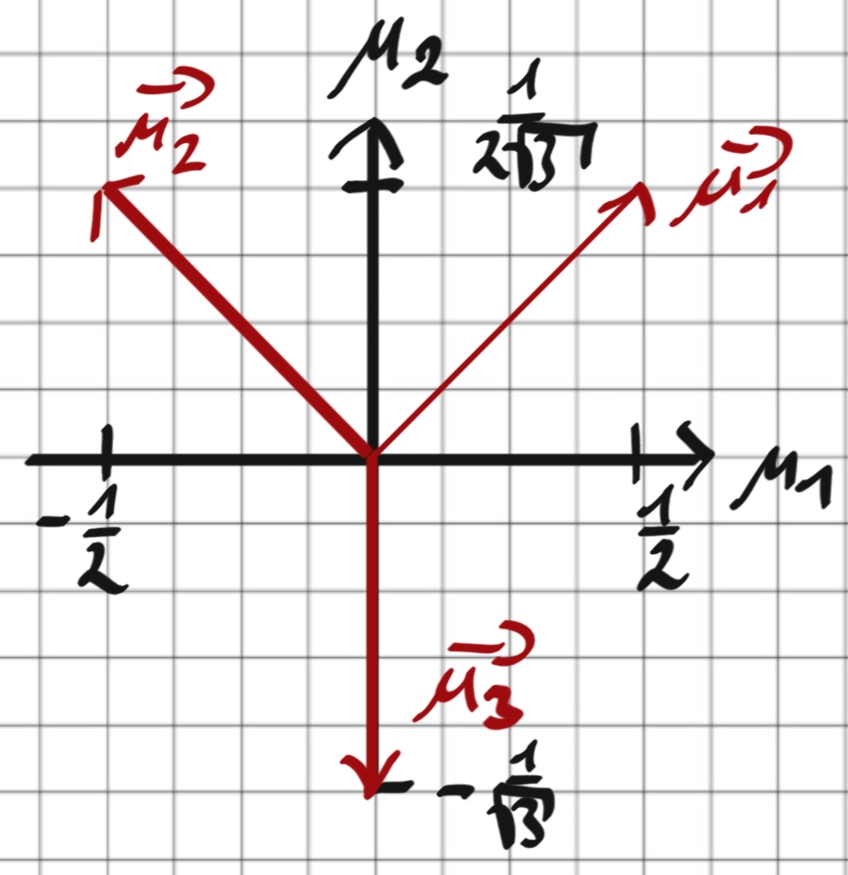
\includegraphics[width = 0.35 \textwidth]{CU_mu.jpg}
  \caption{weightvectors der CU der SU(3).}
  \label{fig:weightvectors}
\end{figure}
\subsection{Flavour SU(3)}
Hier wird in Abbildung \ref{fig:weightvectors} auf die $x$-Achse der Isospin 
aufgetragen.
Also entsprechen die Komponenten von $H_1$ dem Isospin $I_3$.
Auf der $y$-Achse wird die Hyperladung $Y$ reskaliert mit $\sfrac{2}{\sqrt{3}}$ aufgetragen, also enspricht 
$H_2$ der Hyperladung bis auf den Vorfaktor. 
Prinzipiell wird jedem weightvector einfach nur ein Quark zugeordnet (s. Abb. \ref{fig:quark}).
\begin{figure}
  \centering
  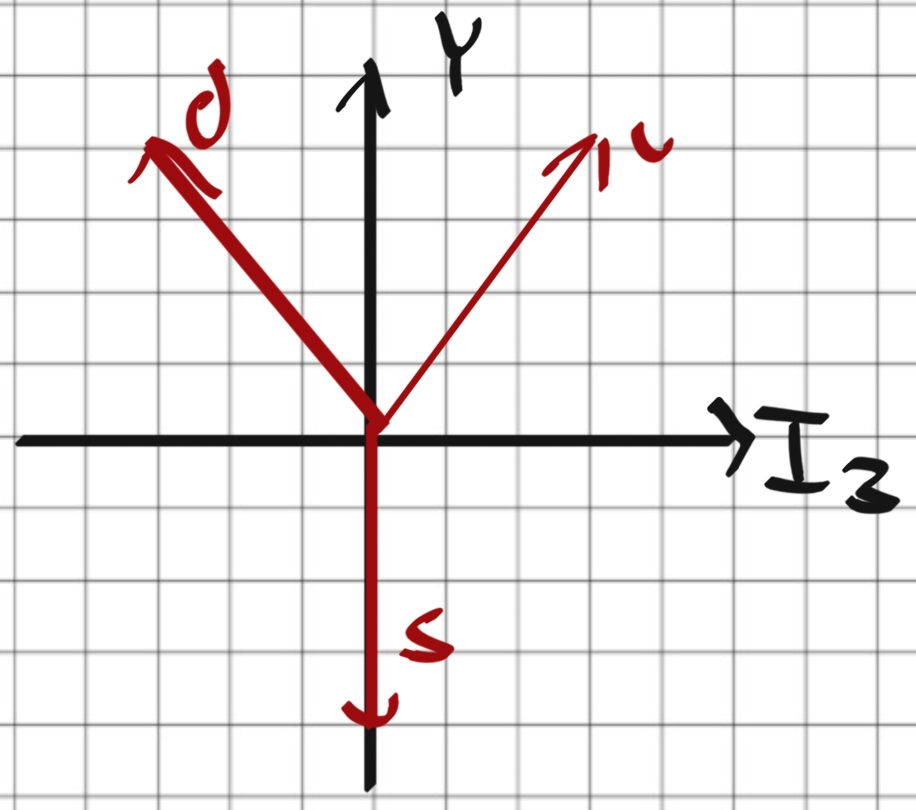
\includegraphics[width = 0.35 \textwidth]{Quark.jpg}
  \caption{Hyperladung-Isospin-Diagramm der Quarks.}
  \label{fig:quark}
\end{figure}
Bei der SU(N) mit $N \geq 3$ gibt es noch die Darstellung 
\begin{equation*}
  U^* = (1 + \frac{\lambda_a\theta^a}{2})^* = (1 - \frac{\lambda_a^*\theta^a}{2})
\end{equation*}
mit $T_a^* =\frac{-\lambda_a^*}{2} = \frac{\lambda_a^{\text{T}}}{2}$.
Die Antiquarks transformieren unter der Darstellung $U^*$.
Analog zu den Quarks lassen sich dazu wieder die weightvectors aufstellen und jedem 
eine Antiquark zuordnen, womit die Abbildung \ref{fig:antiquark} entsteht.
\begin{figure}
  \centering
  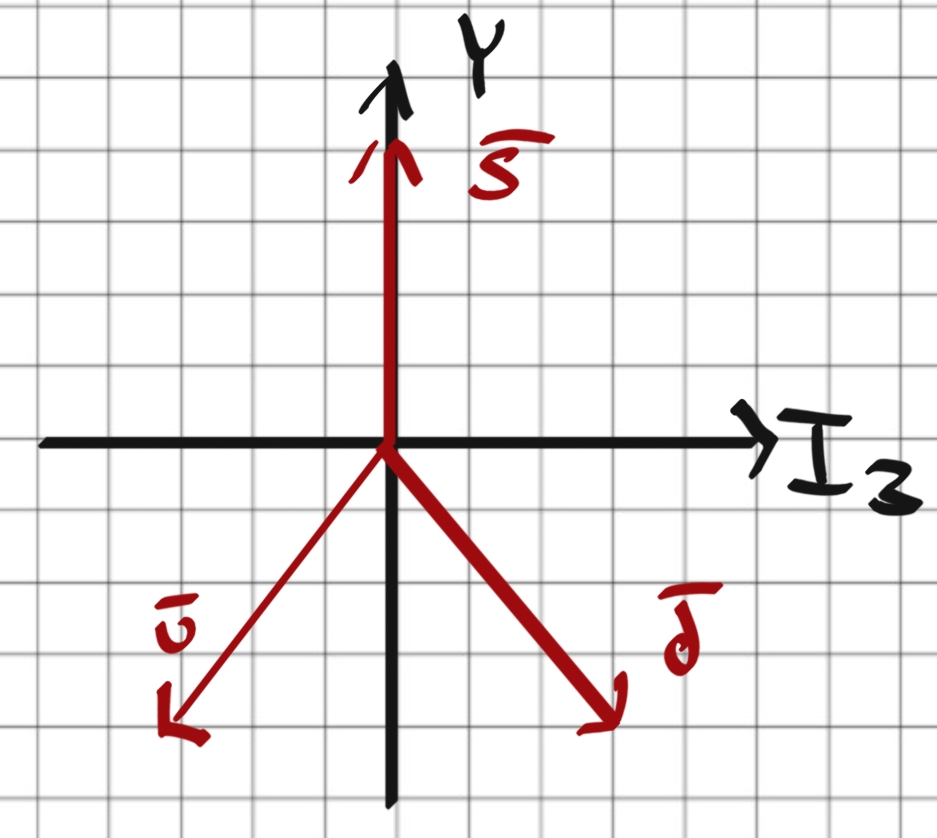
\includegraphics[width = 0.35 \textwidth]{antiquark.jpg}
  \caption{Hyperladung-Isospin-Diagramm der Antiquarks.}
  \label{fig:antiquark}
\end{figure}








\end{document}
